\chapter{Implementacja}
\label{cha:implementation}

\section{Architektura rozwiązania}

\begin{figure}[!ht]
	\begin{center}
		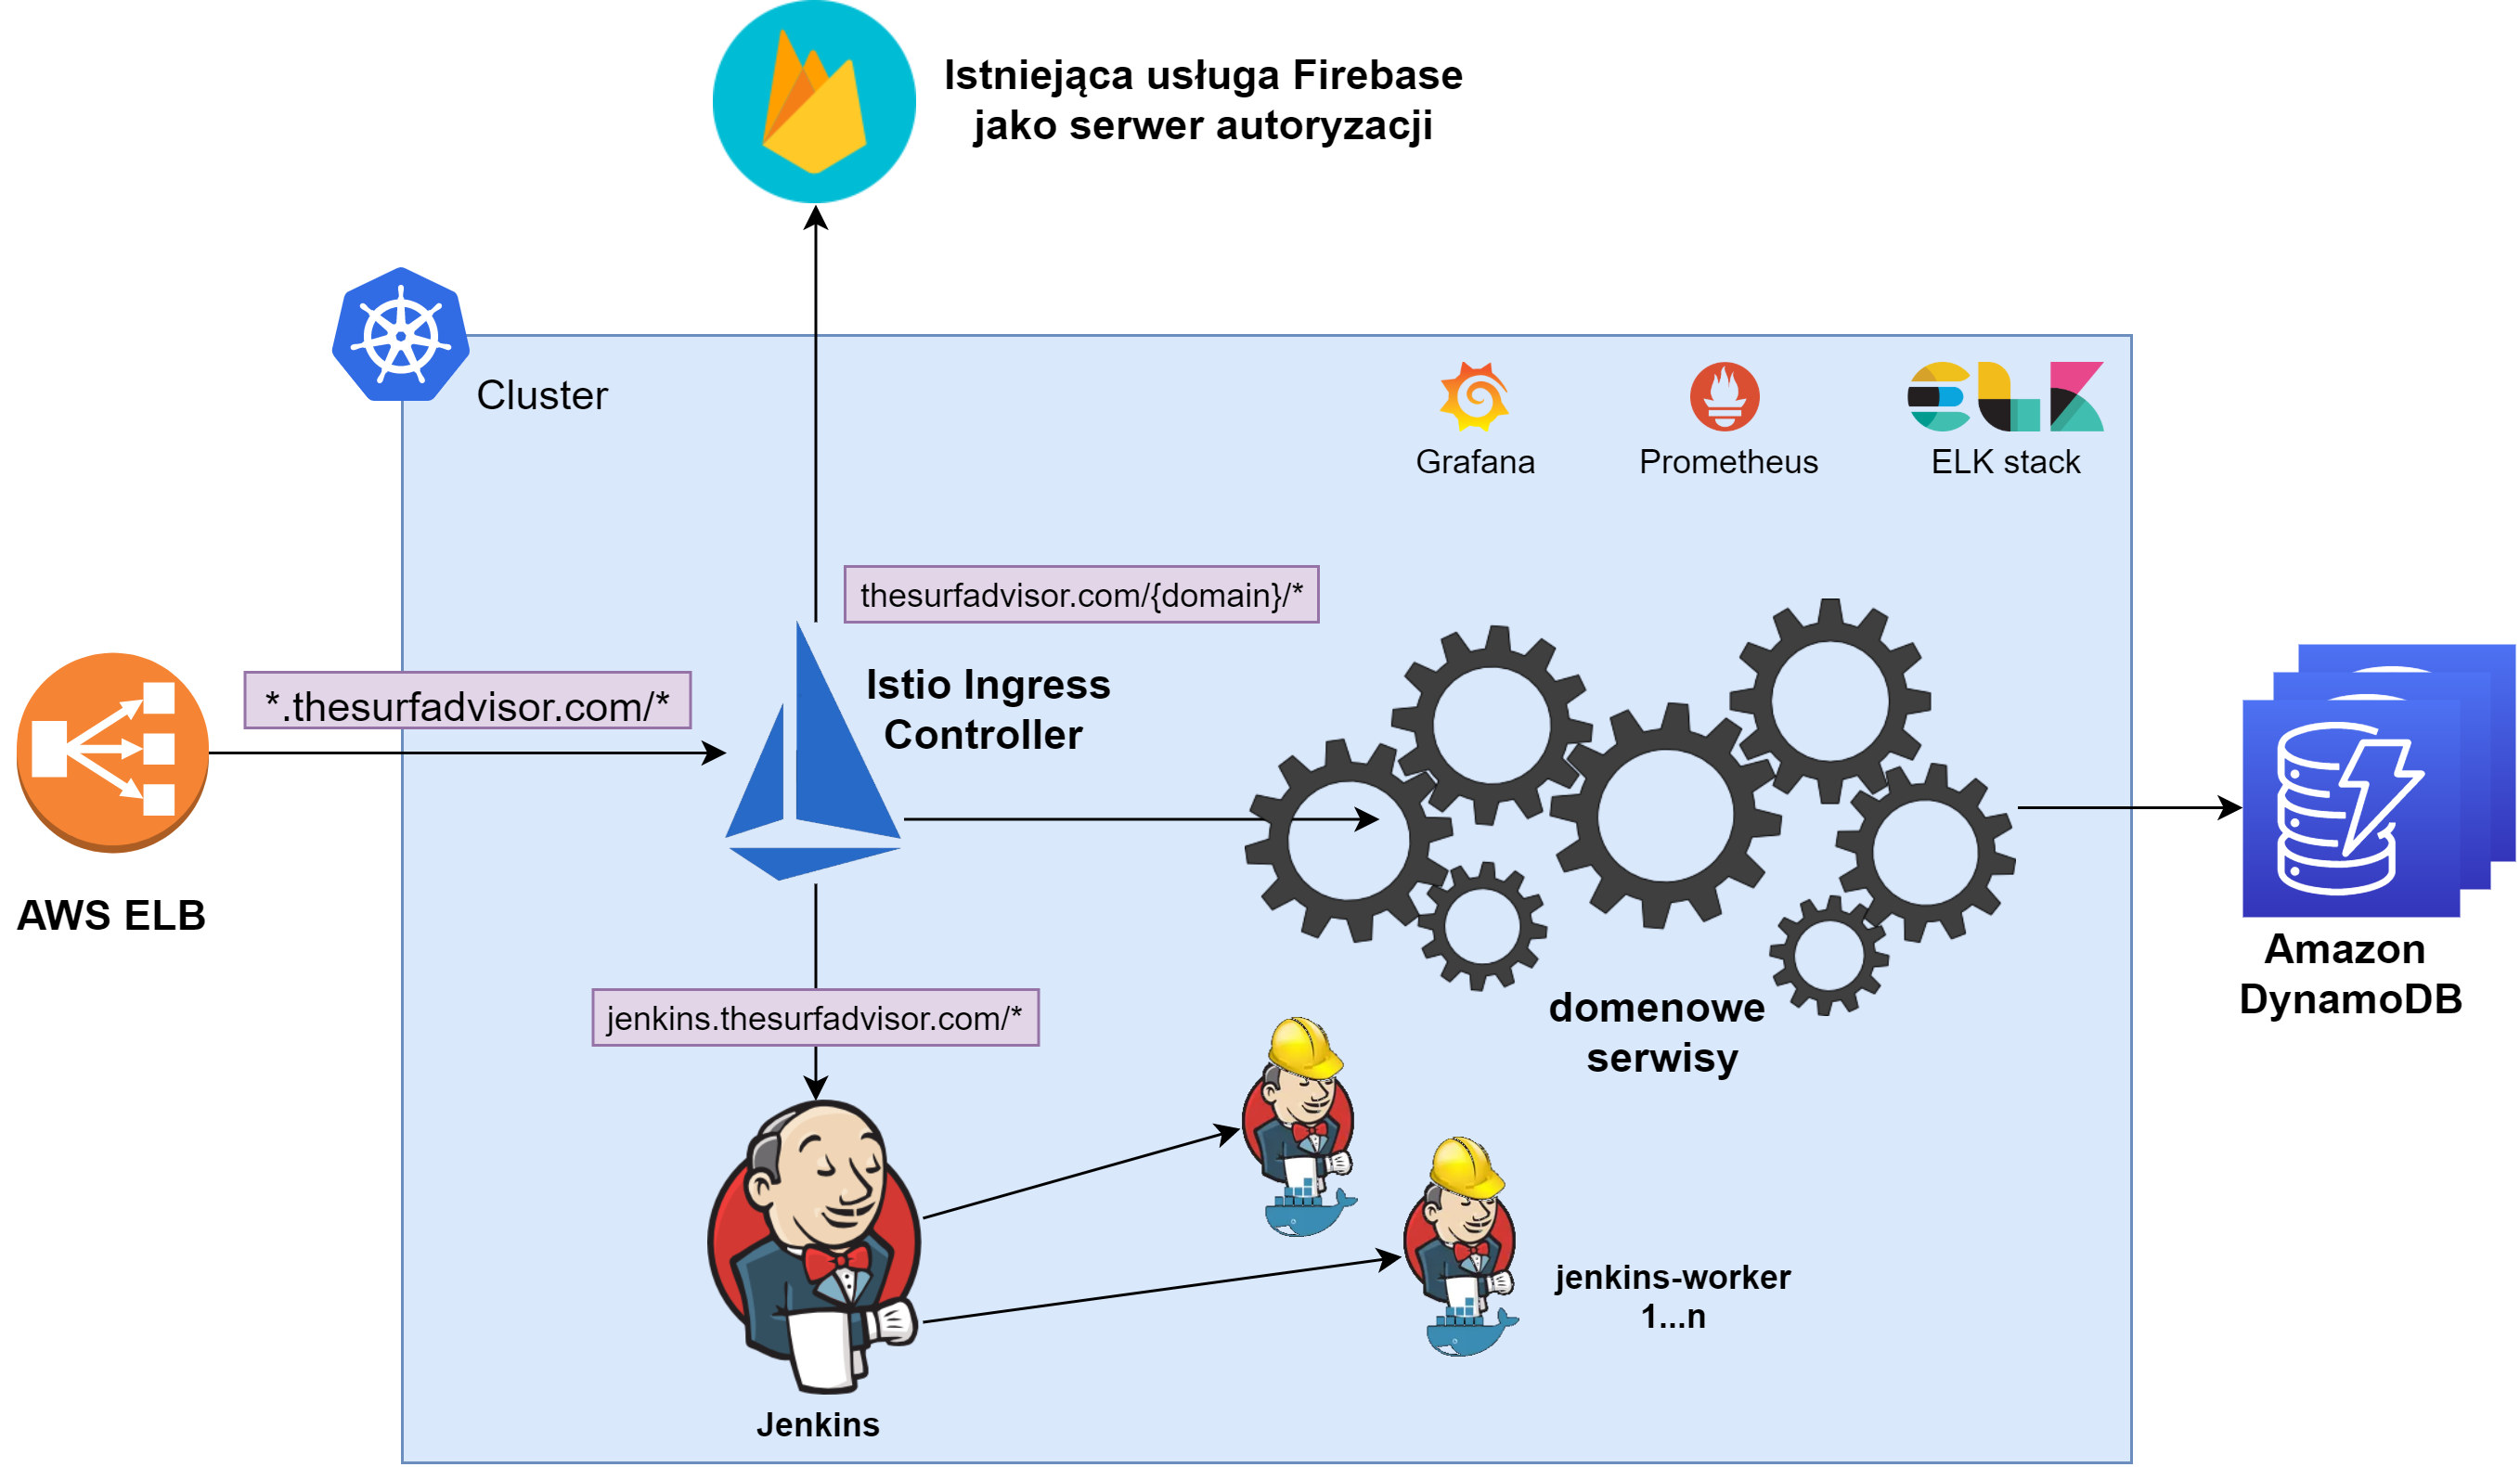
\includegraphics[width=1\textwidth]{img/surf-cluster}
	\end{center}
	\caption{Cluster nowych usług SurfAdvisor}
\end{figure}

\cw{Cluster} nowych usług SurfAdvisor w spoczynku składa się z: 

\begin{itemize}
    \item
    1 x master \cw{Node} - EC2 \textbf{m3.medium} \emph{(1 vCPU \& 3.75 GiB RAM)}

    \item
    2 x worker \cw{Node} - EC2 \textbf{t3.medium} \emph{(2 vCPU \& 4 GiB RAM)}
\end{itemize} 

W przypadku zwiększenia natężenia ruchu liczba \cw{Node}'ów jest skalowana by sprostać wymaganiom.
Pod globalnie dostępną domeną \textbf{thesurfadvisor.com} kryje się \emph{Load Balancer} utrzymywany przez AWS.
Stanowi on jedyny punkt dostępu, cały ruch jest następnie obsługiwany przez Istio \emph{Ingress Controller}.
Autoryzacja zintegrowana jest z istniejącym systemem Firebase. Każdy domenowy serwis uderza do własnej bazy danych DynamoDB.

Jako administrator możemy się dostać do subdomen takich jak:

\begin{itemize}
    \item
    \emph{\textbf{jenkins}.thesurfadvisor.com}\\ 
    Jenkins \emph{WEB UI} pracującego wewnątrz \cw{Cluster}'a

    \item
    \emph{\textbf{grafana}.thesurfadvisor.com}\\
    Grafana \emph{WEB UI} śledząca metryki stanu technicznego

    \item
    \emph{\textbf{kibana}.thesurfadvisor.com}\\
    Kibana \emph{WEB UI} do wygodnego przeszukiwania logów
\end{itemize} 



\section{Aplikacje biznesowe}

\begin{figure}[!ht]
	\begin{center}
		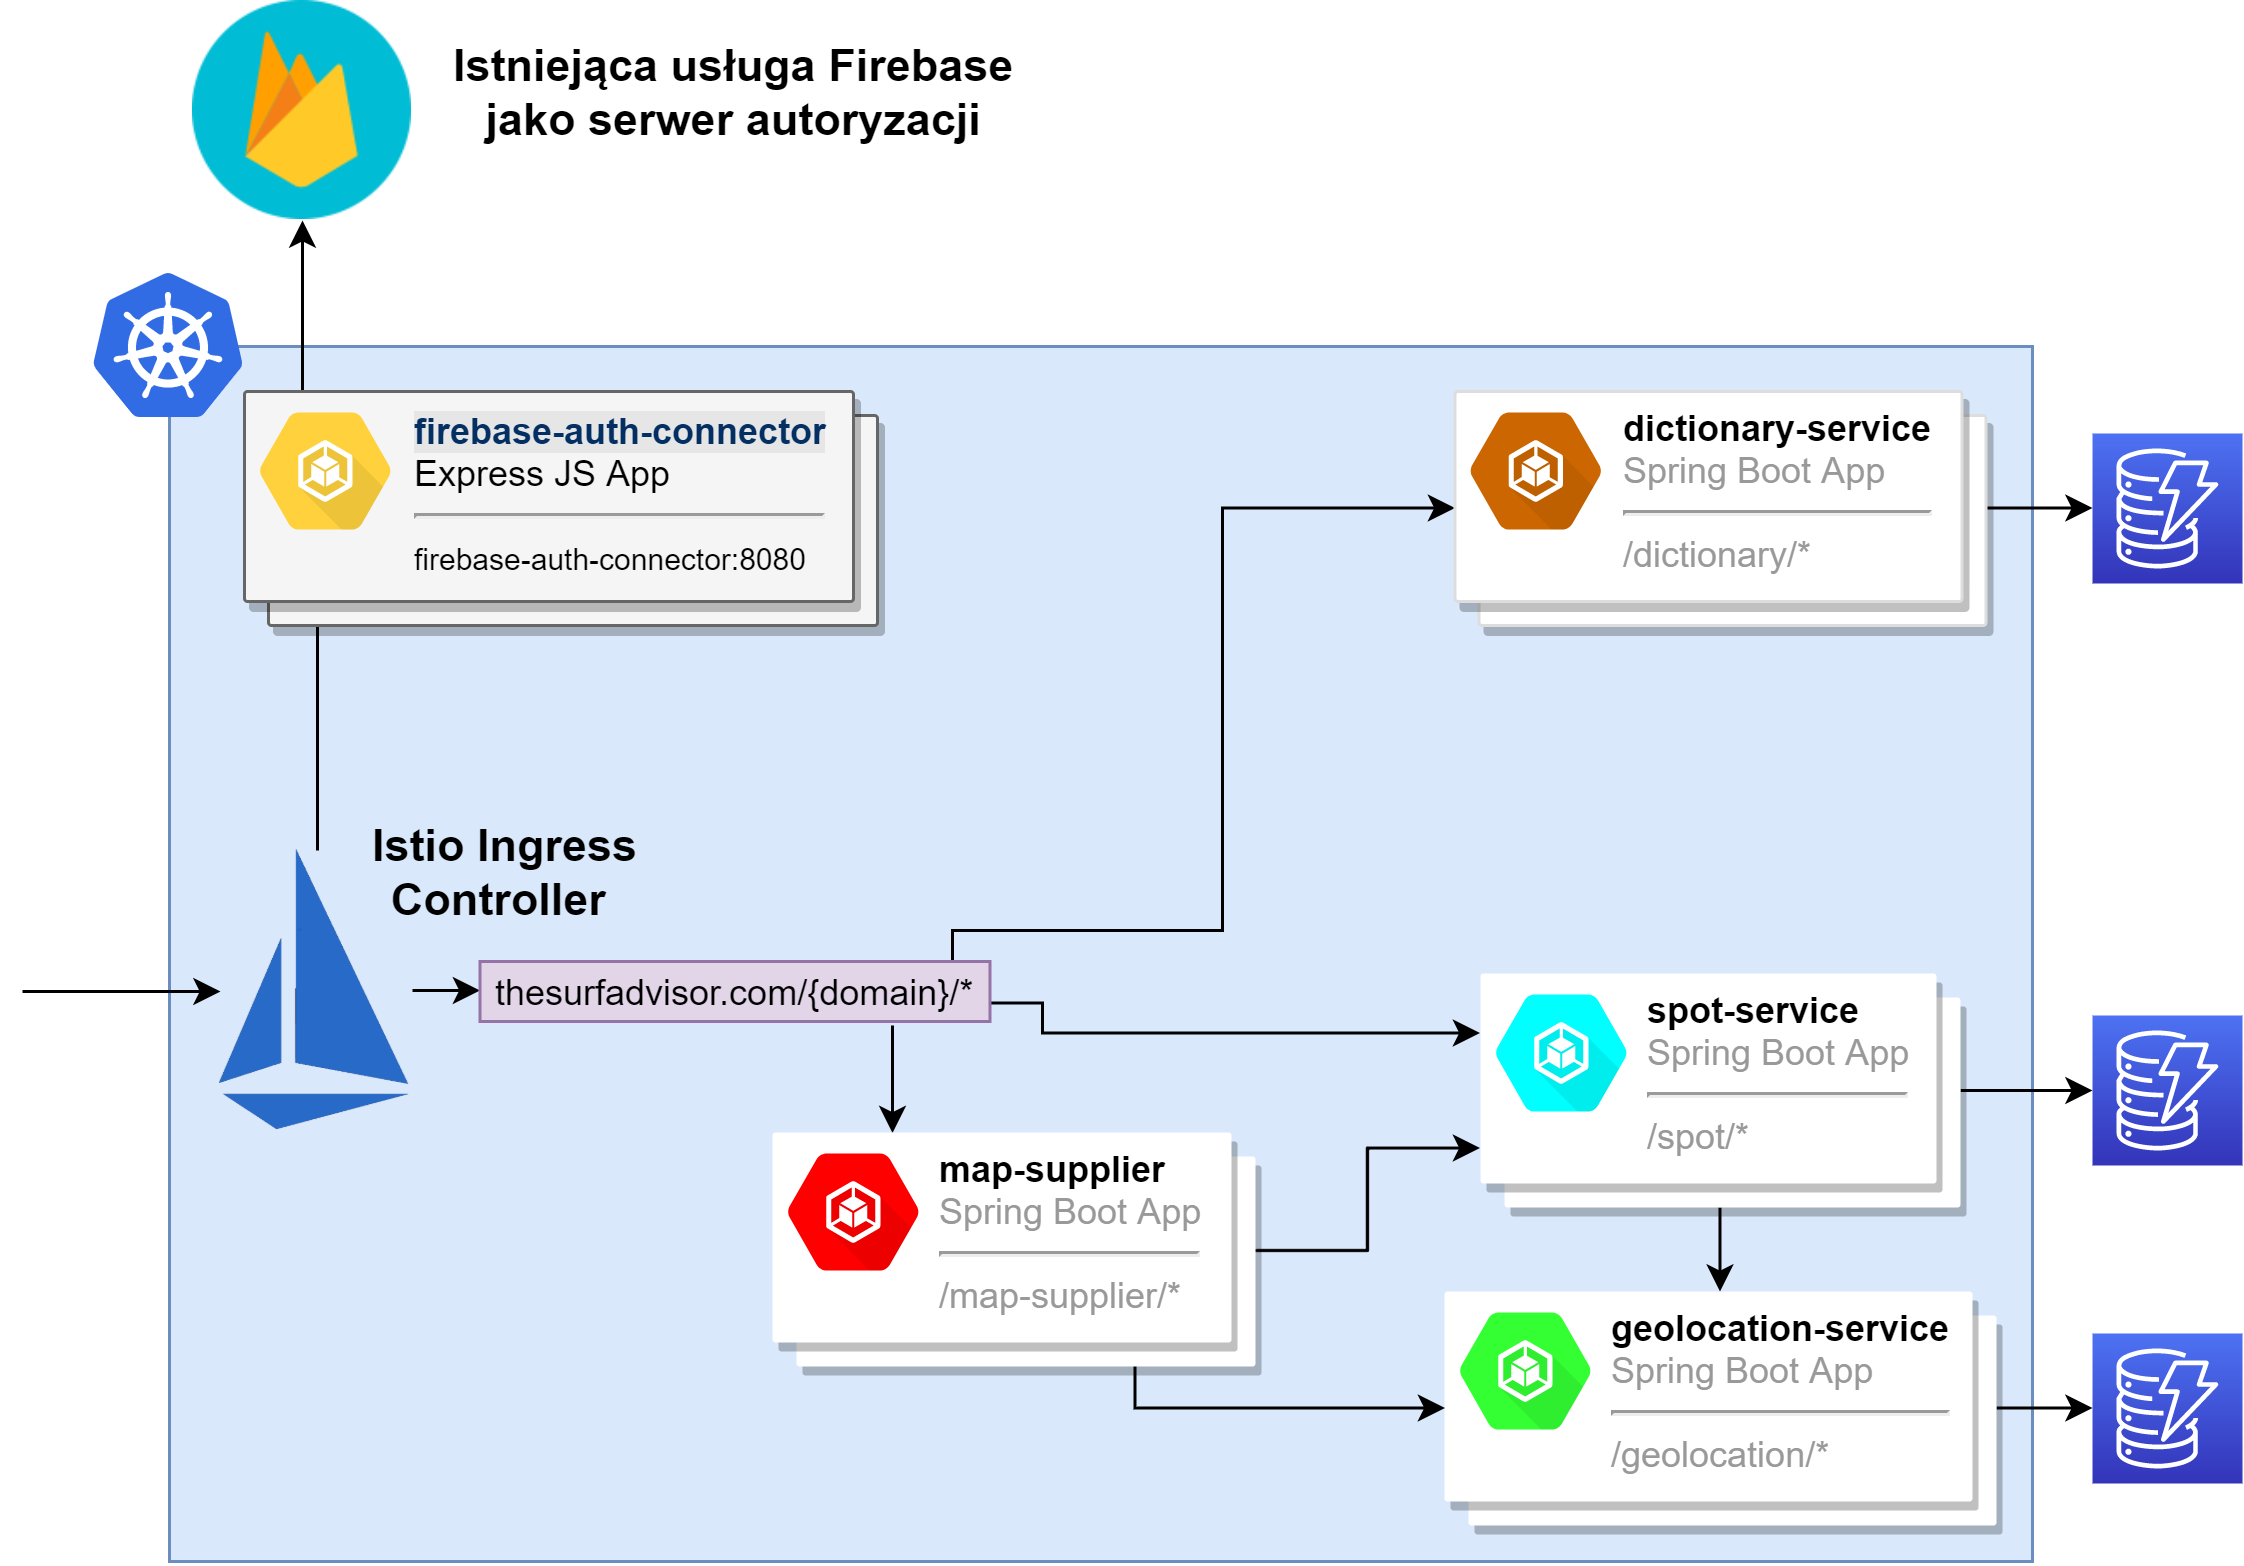
\includegraphics[width=1\textwidth]{img/surf-services}
	\end{center}
    \caption{Zbliżenie na domenowe serwisy SurfAdvisor}
    \label{domain-services}
\end{figure}

\begin{itemize}
    \item
    \textbf{firebase-auth-connector}\\ 
    Warstwa pośrednia pomiędzy Istio \emph{Ingress Controller} a istniejącym serwisem Firebase.
    
    \item
    \textbf{dictionary-service}\\ 
    Repozytorium literałów wyświetlanych w aplikacji mobilnej.

    \item
    \textbf{geolocation-service}\\ 
    Wiedza o położeniu obiektów na kuli ziemskiej.

    \item
    \textbf{spot-service}\\ 
    Atlas spotów - miejsc do uprawiania sportu wodnego.

    \item
    \textbf{map-supplier}\\ 
    Agreguje resztę serwisów związanych z mapą, by wydajniej obsłużyć aplikacje mobilną.
\end{itemize} 




\section{IaC - Infrastructure as Code}

Jest to podejście do zarządzania infrastrukturą \emph{(siecią, wirtualnymi maszynami, kontenerami etc.)} poprzez pliki tekstowe, 
których treść w sposób jednoznaczny definiuje potrzebne zasoby. 
Taką deklaratywną formę konfiguracji bardzo łatwo można śledzić poprzez ten system kontroli wersji co ten używany wokół kodu aplikacji.
IaC jest odpowiedzią na problem różnic pomiędzy środowiskami narastającymi jeszcze bardziej z czasem, jakie powodowały ich manualne imperatywne modyfikacje.
Założeniem IaC jest \textbf{idempotentność} wdrożeń definicji z plików - za każdym razem rezultatem ma być takie samo środowisko \cite{iac-ms}.

W projekcie realizuje tę koncepcję stawiając cały system w czterech krokach. 
Pierwsze trzy stawiają \cw{Cluster} na AWS, są w pełni zautomatyzowane: \emph{CloudFormation}, \emph{Kops} i \emph{Kubernetes}.
Ostatni wdraża domenowe aplikacje, wymaga paru kliknięć w konsoli webowej \emph{Jenkins}'a. 

\subsection{CloudFormation}
\label{iac:cf}

\begin{figure}[!ht]
	\begin{center}
		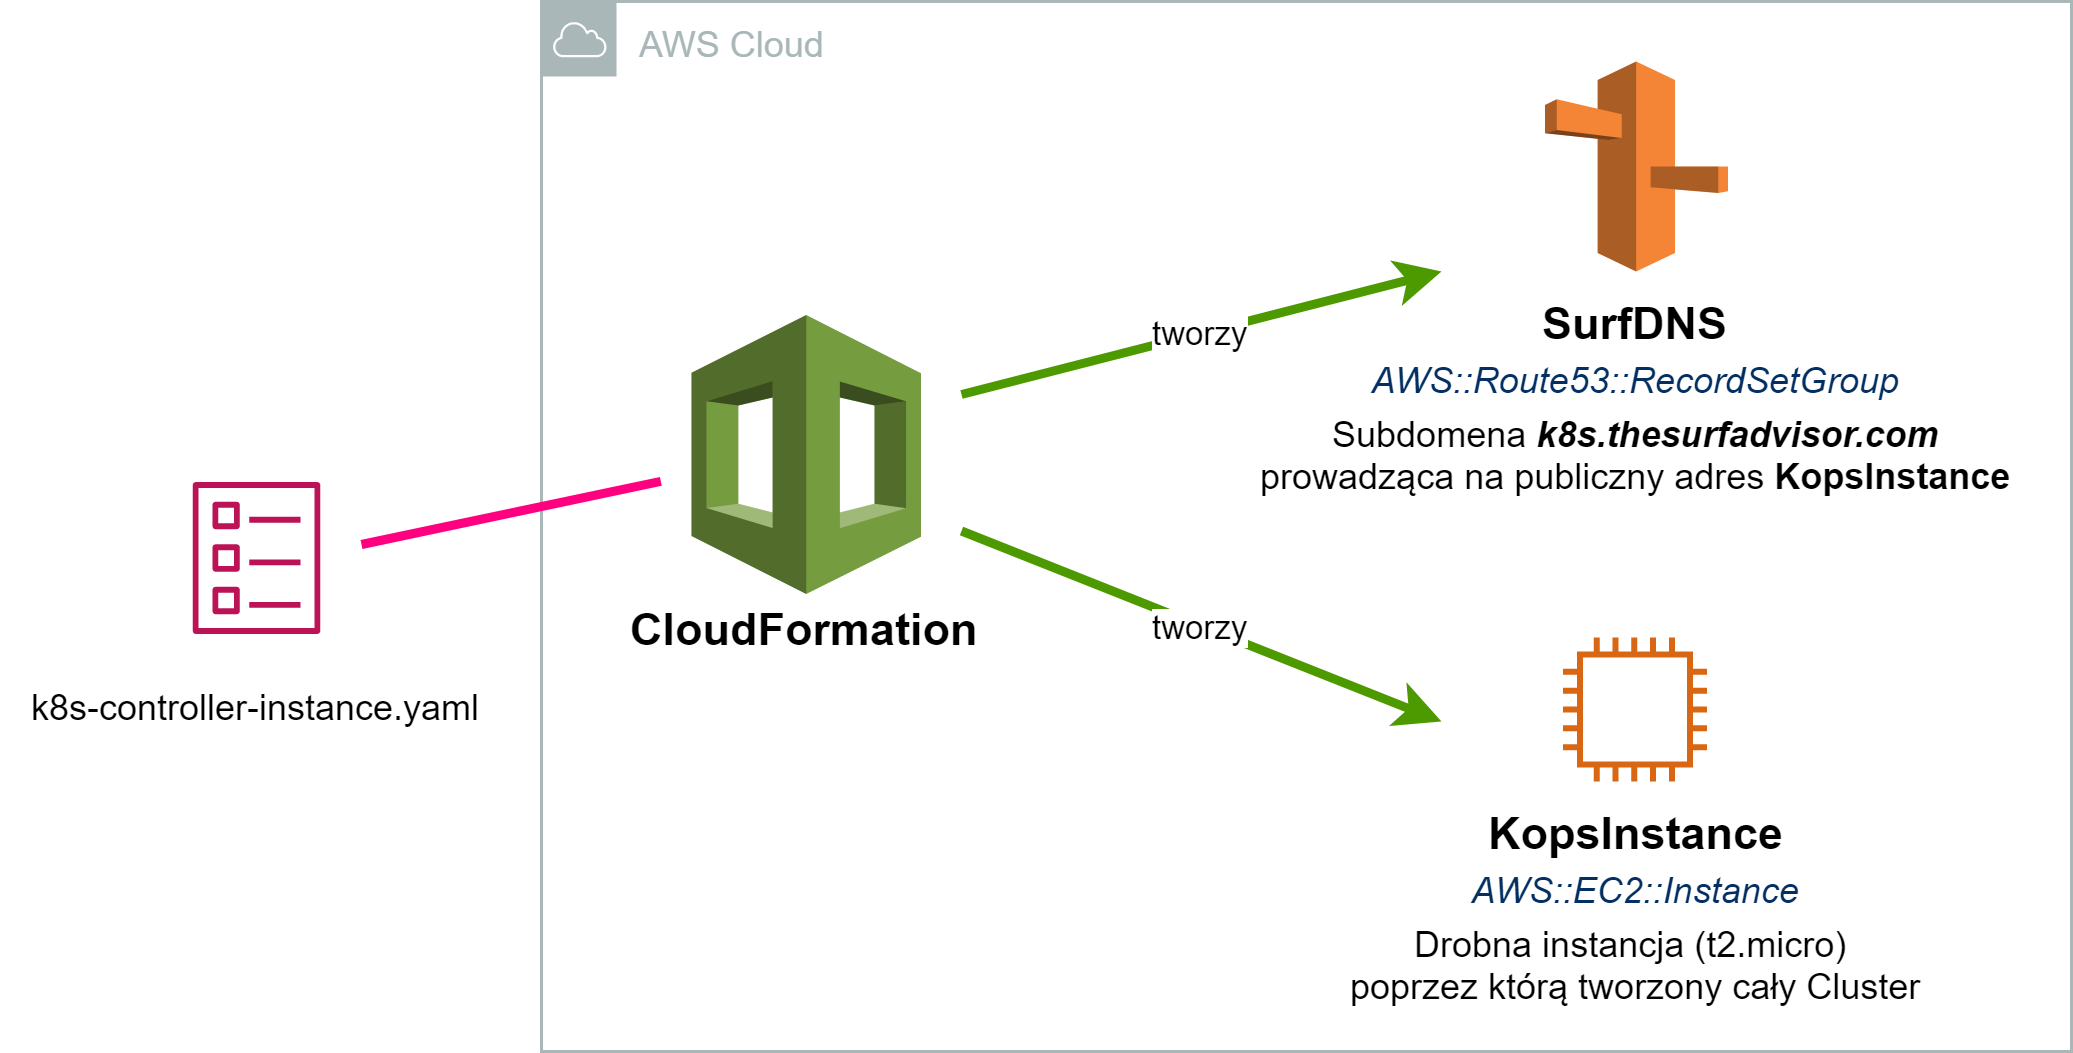
\includegraphics[width=0.9\textwidth]{img/IAC-step1}
	\end{center}
	\caption{Inicjacja Cluter'a SurfAdvisor - 1. CloudFormation}
\end{figure}

Najistotniejszym plikiem CloudFormation w projekcie jest ten inicjujący drobną instancję przeznaczoną do zarządzania docelowym \cw{Cluster}'em.
Plik \cw{k8s-controller-instance.yaml} definiuje głównie: 

\begin{itemize}
    \item
    \textbf{KopsInstance} - drobna instancja linuxa 
    
    \item
    \textbf{SurfDNS} - subdomena oszczędzająca znajomości dokładnego adresu IP \emph{(np. w razie potrzeby ssh)}
\end{itemize} 

Kluczowe znaczenie ma możliwość definicji \emph{\textbf{UserData}} - skryptu \emph{bash} wykonywanego zaraz po starcie instancji. 
Zdefiniowałem w nim polecenia:

\begin{itemize}
    \item
    ściągnięcia dalszych instrukcji \emph{bash} z S3

    \item
    instalacji potrzebnych narzędzi \emph{(kops, kubectl, helm)}
    
    \item
    zbudowania \cw{Cluster}'a poprzez \emph{kops} \emph{(\ref{iac:kops})}

    \item
    wdrożeniu pomocniczych \cw{Service}'ów poprzez \emph{kubectl} \& \emph{helm} \emph{(\ref{iac:kubectl})}
\end{itemize} 

\subsection{Kops}
\label{iac:kops}

\begin{figure}[!ht]
	\begin{center}
		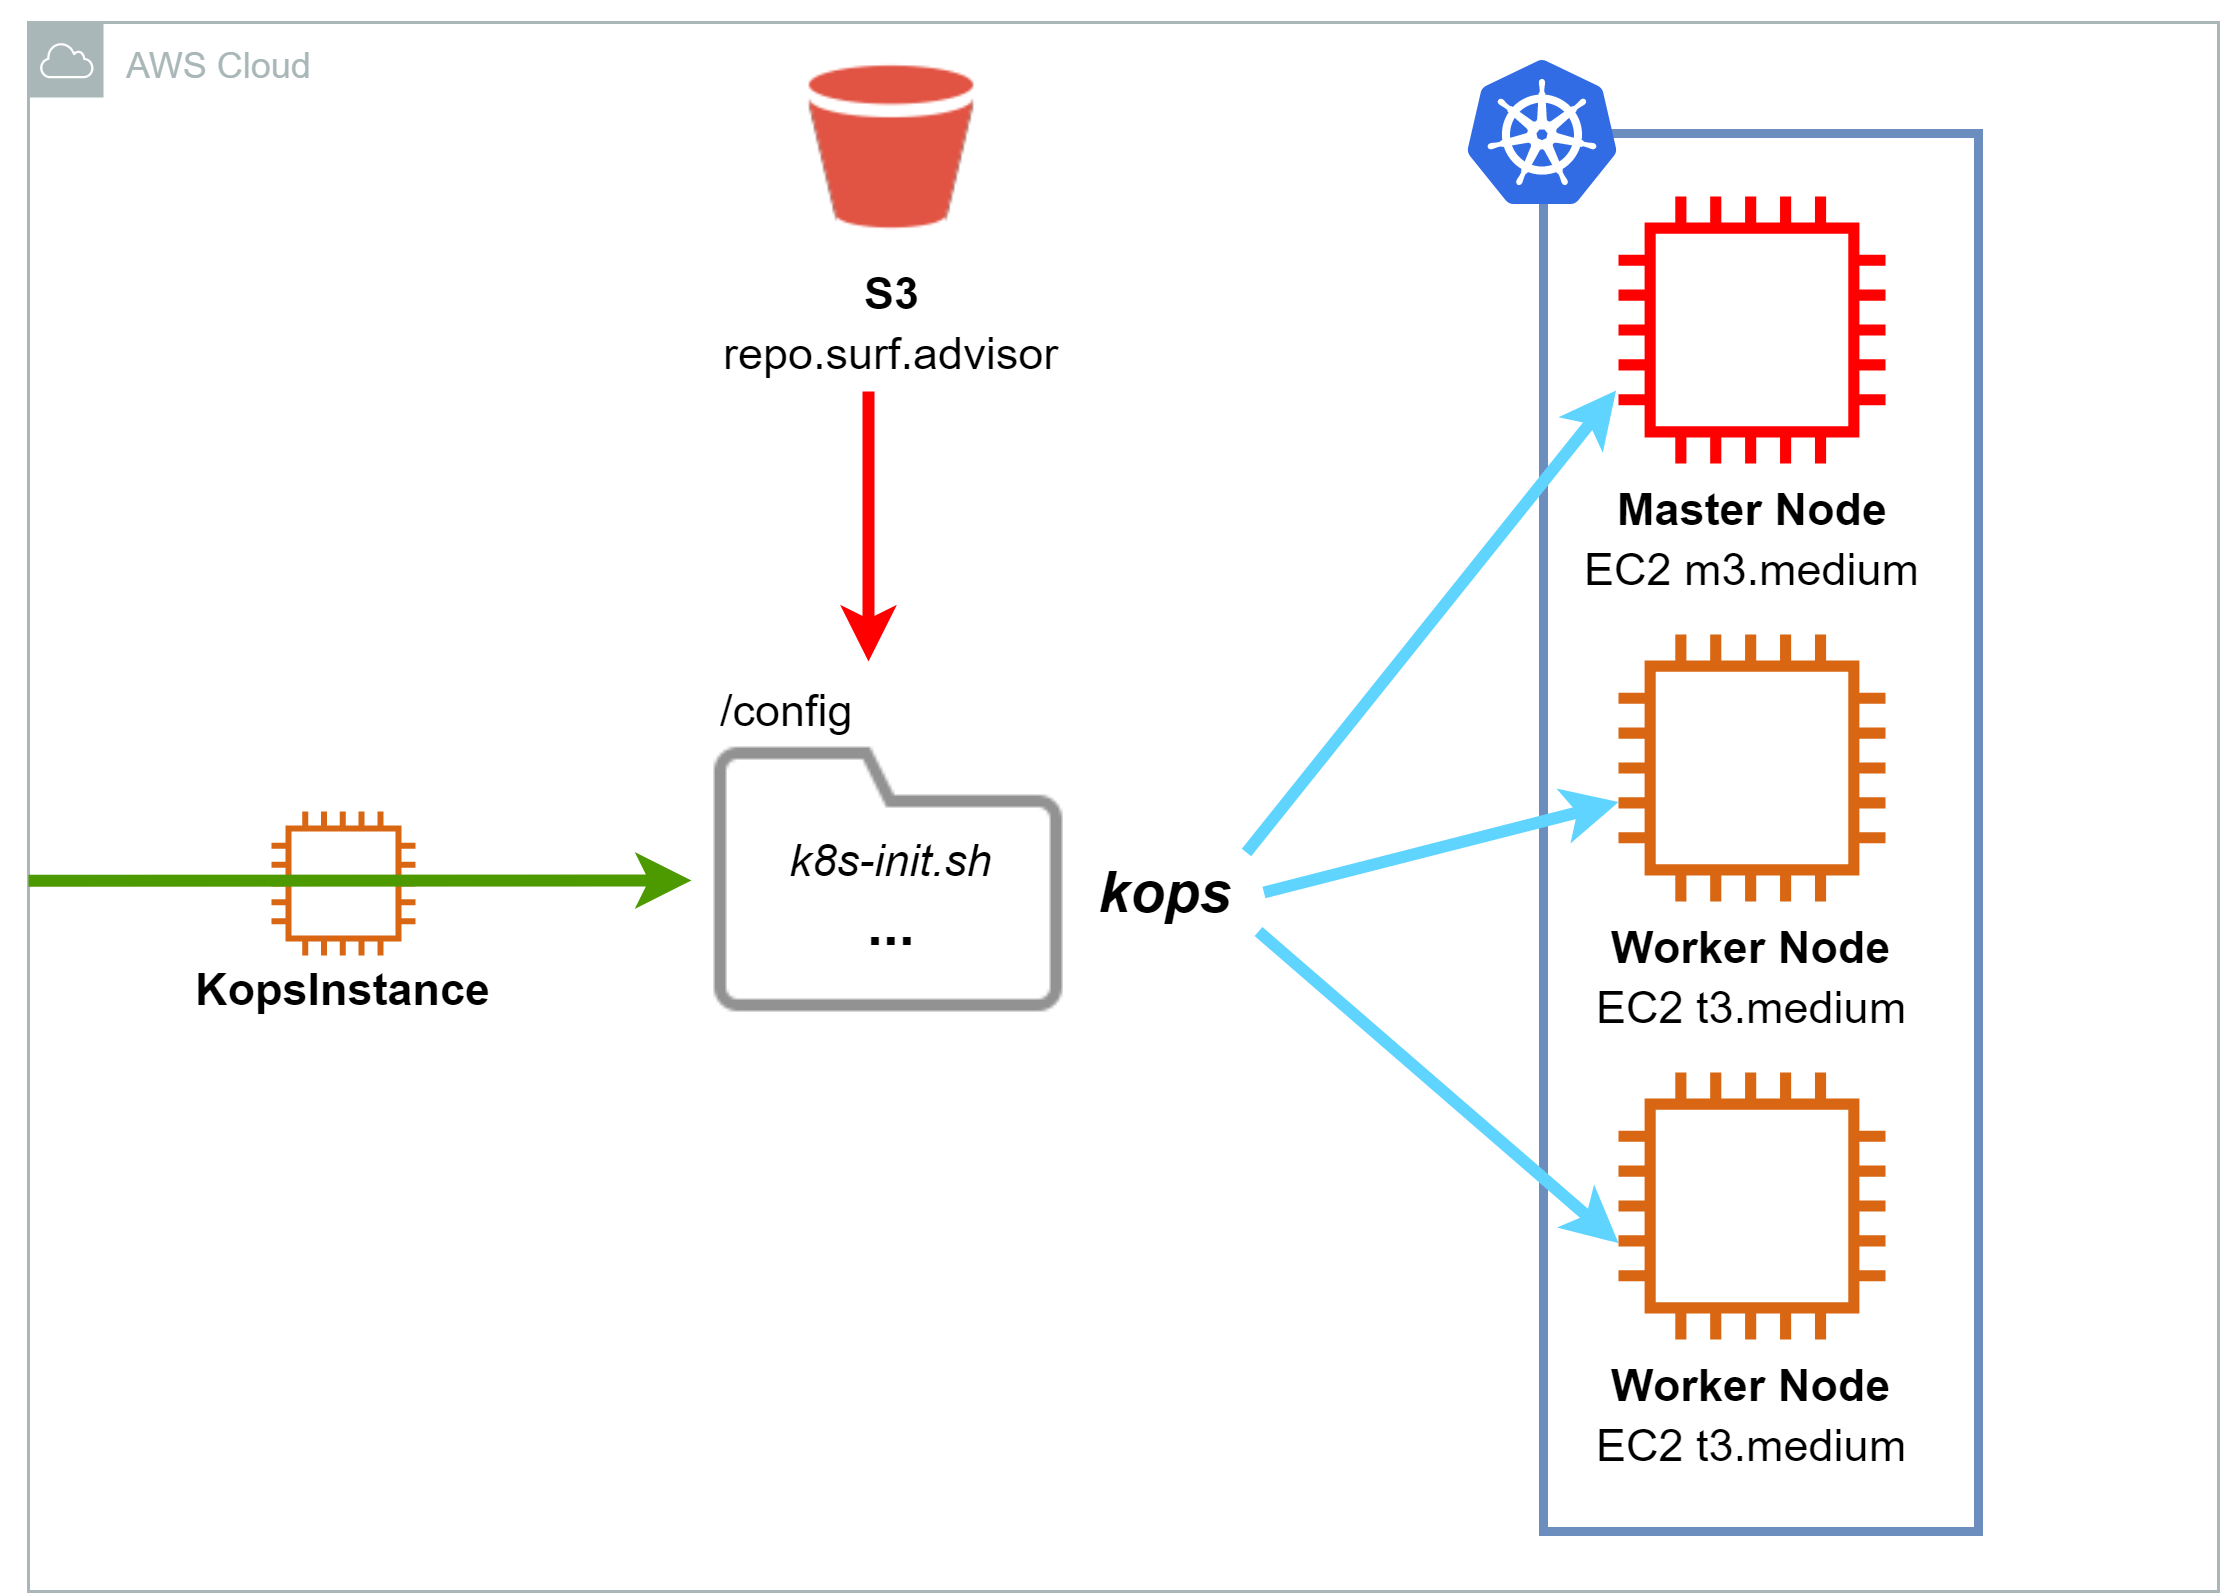
\includegraphics[width=0.95\textwidth]{img/IAC-step2}
	\end{center}
	\caption{Inicjacja Cluter'a SurfAdvisor - 2. Kops}
\end{figure}

\emph{kops} to open-source CLI do budowania \cw{Cluster}'ów Kubernetes na platformie AWS \cite{kops-k8s}.
Stanowi alternatywę dla stosunkowo drogiego na start oficjalnego rozwiązania - EKS \cite{eks-pricing}.

Przy użyciu tego narzędzia dalszy ciąg skryptów, uruchomionych w ramach \emph{UserData} \textbf{KopsInstance} \emph{(\ref{iac:cf})}, buduje \cw{Node}'y składające się na \cw{Cluster}.


\subsection{Kubernetes}
\label{iac:kubectl}

\begin{figure}[!ht]
	\begin{center}
		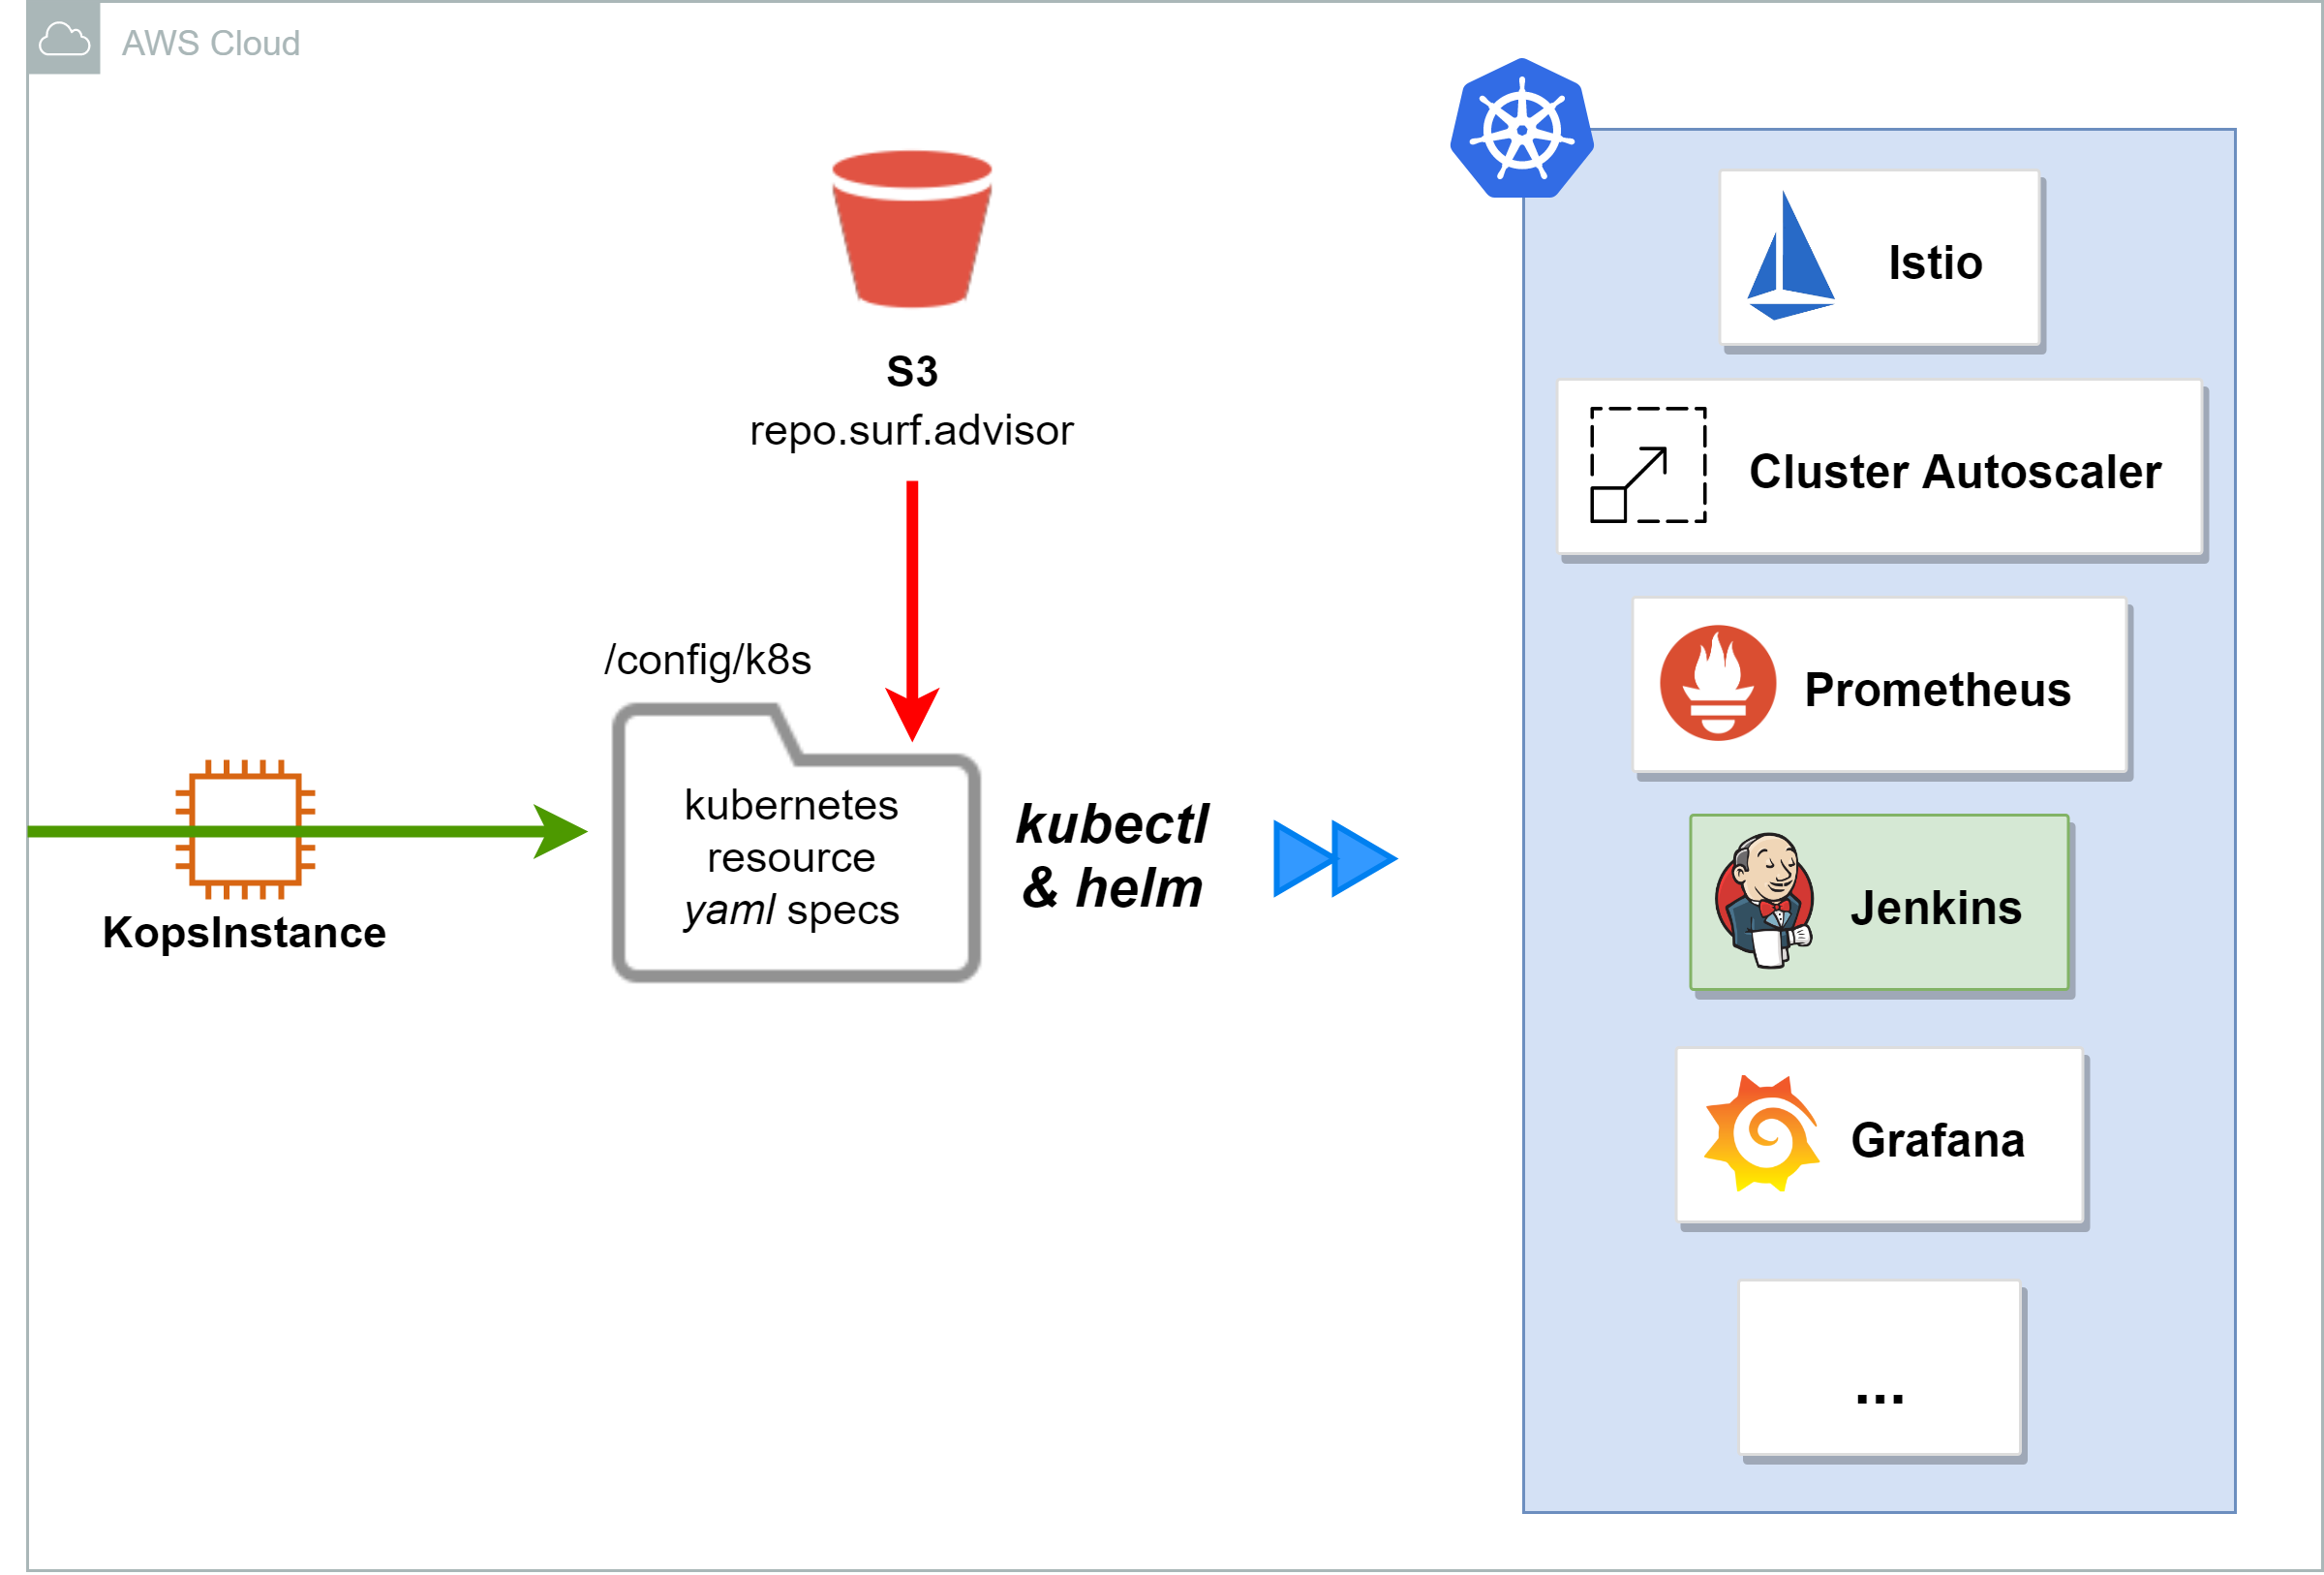
\includegraphics[width=1\textwidth]{img/IAC-step3}
	\end{center}
	\caption{Inicjacja Cluter'a SurfAdvisor - 3. Kubernetes}
\end{figure}

Gdy \emph{kops} skończy już stawiać \cw{Cluster} do akcji wkracza:

\begin{itemize}
    \item
    \emph{\textbf{kubectl}} - oficjalne CLI do operacji na zasobach Kubernetes

    \item
    \emph{\textbf{helm}} - package manager dla Kubernetes
\end{itemize} 

Wdrażane są \cw{Service}'y zaspokajające wymagania bardziej niefunkcjonalne, m.in.:

\begin{itemize}
    \item
    \emph{Jenkins} - który kontynuuje proces inicjacji systemu \emph{[\ref{iac:jenkins}]}

    \item
    \emph{Istio} - sekcja \emph{[\ref{traffic}]}

    \item
    \emph{Prometheus \& Grafana} - monitoring parametrów technicznych \cw{Cluster}'a

    \item
    \emph{Cluster Autoscaler} - rozdział \emph{[\ref{cha:autoscaling}]}
\end{itemize} 


\subsection{Jenkins}
\label{iac:jenkins}

Jenkins jest gotowy do użycia po paru minutach \emph{(wraz ze wszystkimi plugin'ami zdefiniowanymi w pliku konfiguracyjnym)}.
Jedynym manualnym krokiem jaki musimy wykonać jest stworzenie zadania \emph{"Github Organization"}, gdzie podajemy ID naszej organizacji.

\begin{figure}[!ht]
	\begin{center}
		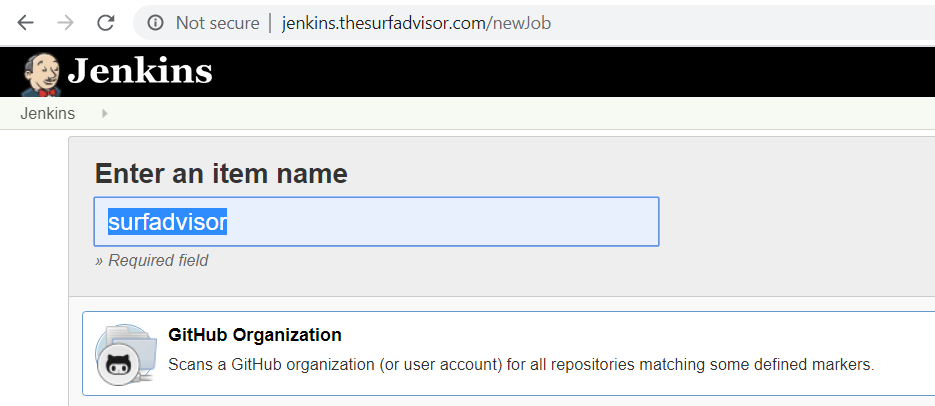
\includegraphics[width=0.8\textwidth]{img/jenkins-new-job}
	\end{center}
	\caption{Jenkins: wdrożenie domenowych serwisów - job "Github Organization"}
\end{figure}

Następnie Jenkins skanuje wszystkie repozytoria widniejące pod daną organizacją i wybiera te zawierące \textbf{\emph{Jenkinsfile}}.
Po chwili będzie dostępna zakładka, na której wylistowane są wszystkie repozytoria spełniające wyżej wymienone kryterium:

\begin{figure}[!ht]
	\begin{center}
		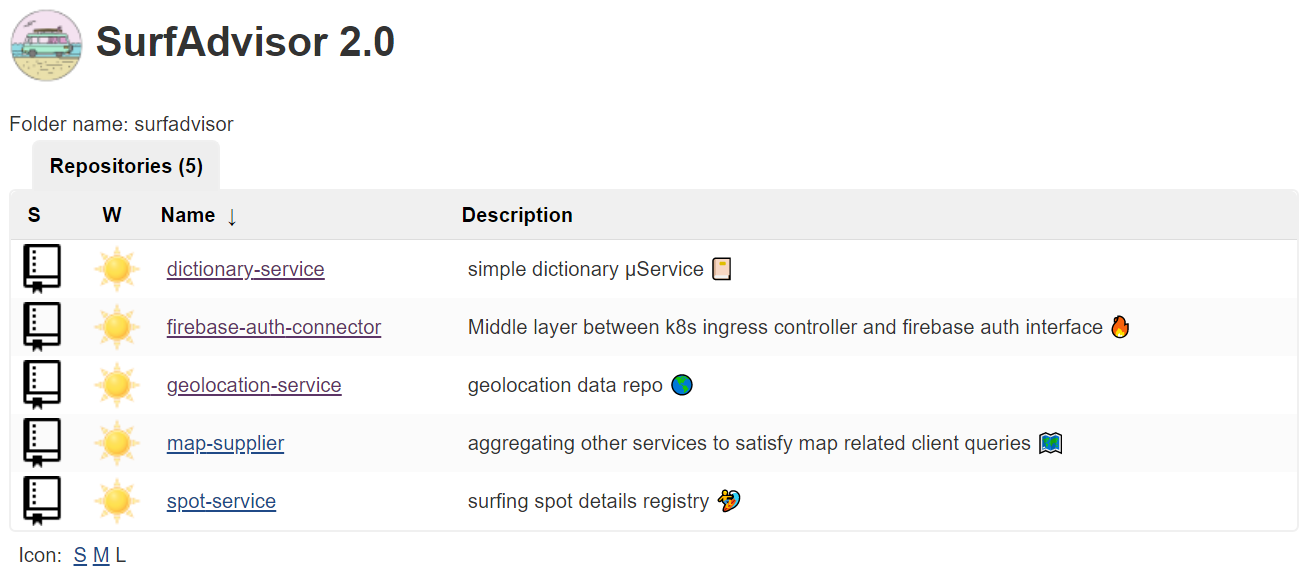
\includegraphics[width=1\textwidth]{img/jenkins-surf-folder}
	\end{center}
	\caption{Jenkins: wdrożenie domenowych serwisów - folder SurfAdvisor}
\end{figure}

Dla każdego z repozytorium Jenkins od razu uruchamia zdefiniowany w \emph{Jenkinsfile} pipeline.
W moim przypadku repozytoria łączy jeszcze obecność dwóch innych plików:
\\\\
\begin{itemize}
    \item
    \emph{\textbf{Dockerfile}} - instrukcja budowy docker image wstawianego potem na DockerHub
    \item
    \emph{\textbf{deploy.yaml}} - deklaracja obiektów Kubernetes: \cw{Service}, \cw{Deployment}, \cw{Pod}, na których stanie dana aplikacja.
    Wdrażane są poprzez \emph{kubectl}.
\end{itemize} 

Poniżej przedstawiony jest wycinek procesowania pipeline dla aplikacji \emph{geolocation-service}.
Dwa końcowe kroki udekorowane są dodatkowo symbolem pliku, na którym polegają.

\begin{figure}[!ht]
	\begin{center}
		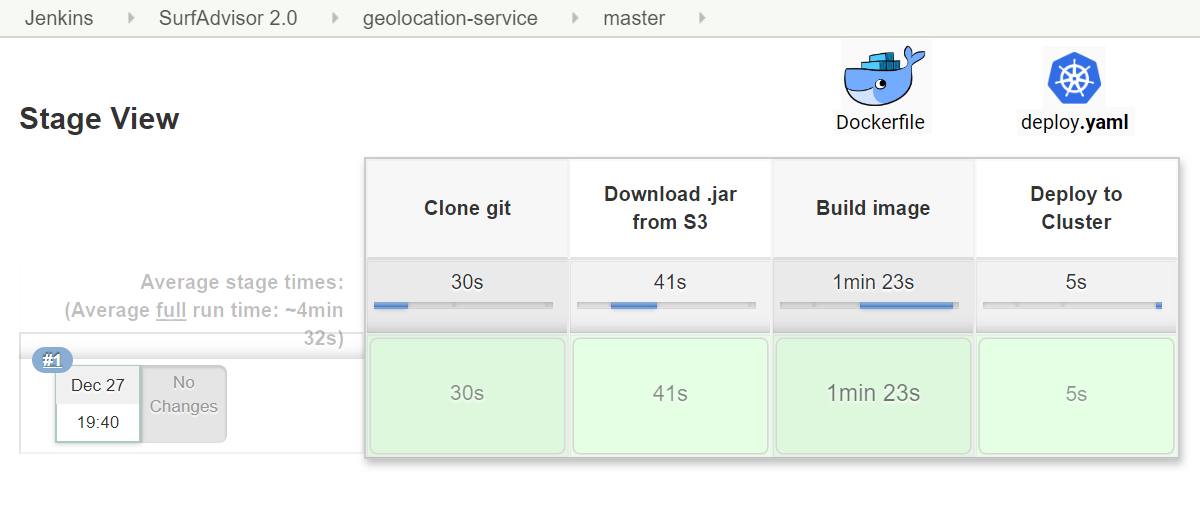
\includegraphics[width=1\textwidth]{img/jenkins-geo-stages}
	\end{center}
	\caption{Jenkins: wdrożenie domenowych serwisów - pipeline}
\end{figure}

\subsection{Usuwanie}

Cały powstały w sposób opisany wyżej \cw{Cluster} wraz ze wszystkimi powiązanymi produktami AWS (\emph{EC2, LoadBalancer, etc.}) usuwa się jedną komendą:

\begin{itemize}
    \item
    \textcolor{blue}{\texttt{kops delete cluster --name \$\{NAME\} --yes}}
\end{itemize} 

Bardzo przydatne na etapie developmentu - usuwamy system kończąc pracę w danym dniu, co przynosi spore oszczędności.

\section{Zarządzanie ruchem i bezpieczeństwo}
\label{traffic}

\begin{figure}[!ht]
    
	\begin{center}
		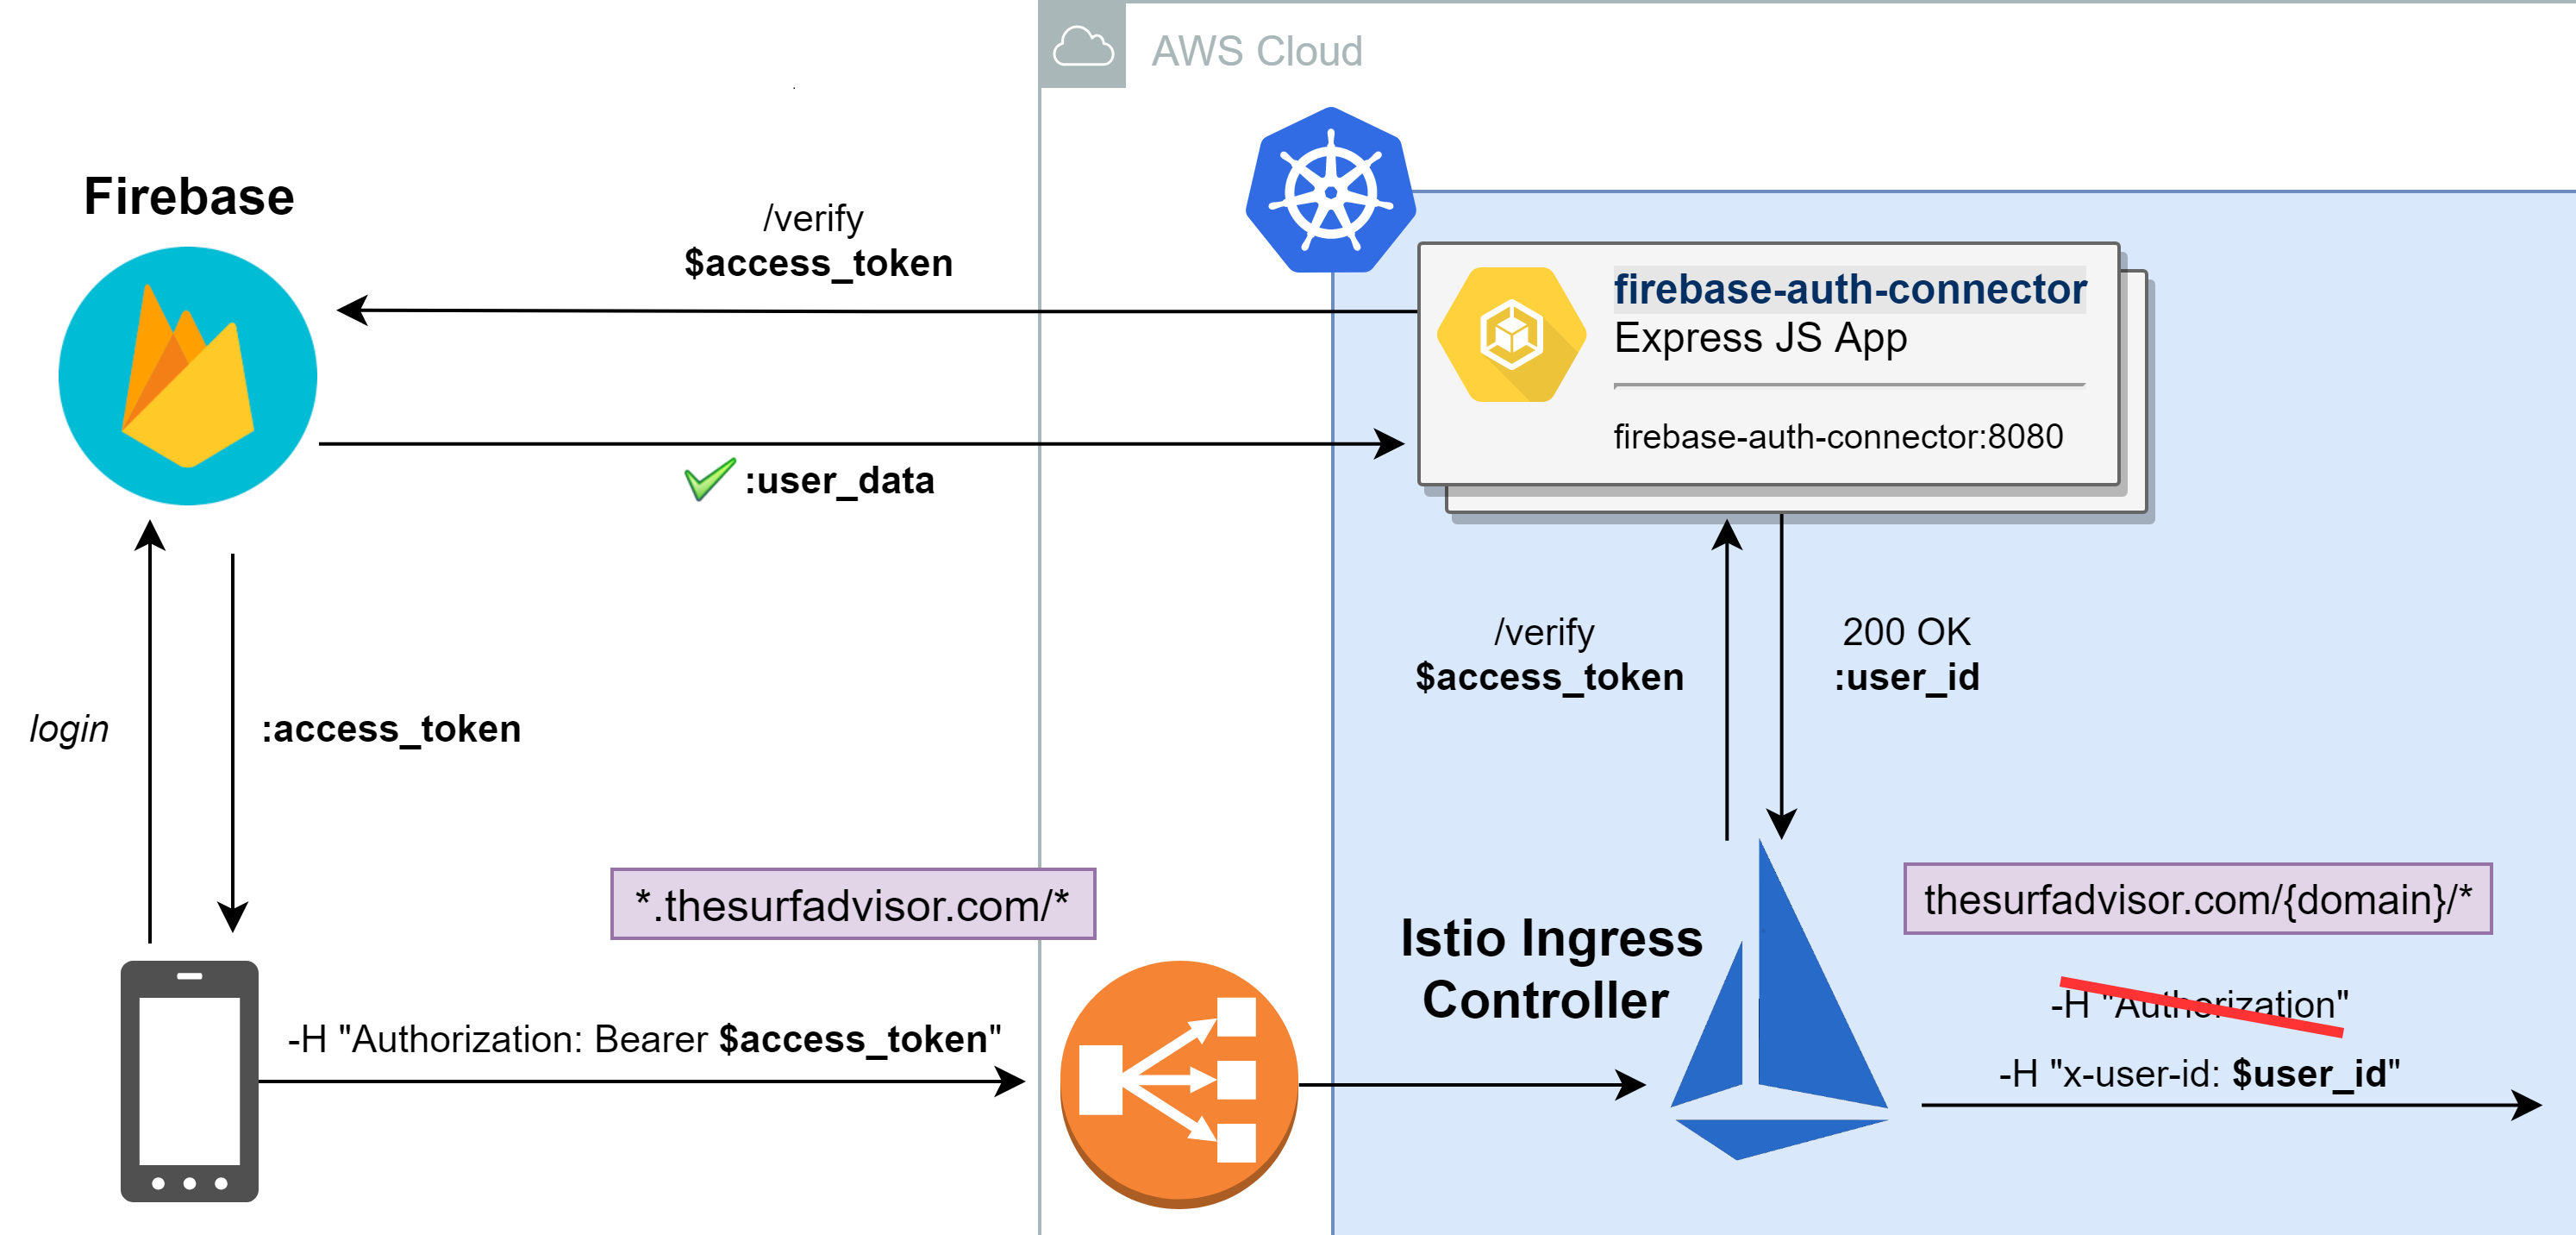
\includegraphics[width=0.93\textwidth]{img/security-flow}
	\end{center}
    \caption{Diagram autentykacji / autoryzacji}
    \label{security-diagram}
\end{figure}

Poprzez ustawienie w Route53 ruch w stronę globalnie dostępnej domeny \emph{\textbf{thesurfadvisor.com}} jest kierowany na Load Balancer, 
który następnie rozrzuca go po \cw{Node}'ach \cw{Cluster}'a.
Na każdym z tych \cw{Node}'ów ruch trafia wpierw do instancji Istio \emph{Ingress Controller}. 
Po pomyślniej autentykacji ruch jest kierowany do odpowiedniego \cw{Service}'u na podstawie ścieżki.
\\\\\\\\
Diagram \ref{security-diagram} ilustruje przebieg autentykacji i autoryzacji:
\begin{enumerate}
    \item
    Proces logowania w aplikacji mobilnej pozostaje bez zmian. Tak jak w starej wersji użytkownik loguje się do Firebase którymś z dostępnych sposobów.

    \item
    Aplikacja mobilna dekoruje zapytania do \emph{thesurfadvisor.com} header'em z tym samym tokenem dostępu, który jest używany do komunikacji z usługami Firebase.

    \item
    Istio \emph{Ingress Controller} deleguje weryfikację nadchodzącego tokena do \cw{Service}'u \textbf{\emph{firebase-auth-connector}}.

    \item
    \emph{firebase-auth-connector} poprzez oficjalne SDK zleca Firebase weryfikację tokena.
    W przypadku sukcesu Firebase zwraca mały zbiór podstawowych danych użytkownika.
    Nasz \cw{Service} zwraca do Istio tylko jego identyfikator, w planach jest dołożenie jeszcze zbioru uprawnień. 

    \item
    Istio usuwa niepotrzebny już header ''Authorization'' i ustawia ''x-user-id'' z identyfikatorem użytkownika.
    W ten sposób dalsze domenowe serwisy są odciążone od implementowania tego aspektu bezpieczeństwa.
\end{enumerate} 



\section{Realizacja wymagań funkcjonalnych}

\subsection{Diagram klas \emph{spot-service} API}

\begin{figure}[H]
	\begin{center}
		\includegraphics[width=1\textwidth]{out/plantuml/spot-api/spot-api.pdf}
	\end{center}
    \caption{Diagram klas \emph{spot-service} API}
    \label{spot-api}
\end{figure}

\subsection{Diagram klas \emph{map-supplier} API}

\begin{figure}[H]
	\begin{center}
		\includegraphics[width=1\textwidth]{out/plantuml/map-supplier-api/map-supplier-api.pdf}
	\end{center}
    \caption{Diagram klas \emph{map-supplier} API}
    \label{ms-api}
\end{figure}


\begin{figure}[H]
	\begin{center}
		\includegraphics[width=0.1\textwidth]{out/plantuml/map-query-flow/map-query-flow-empty.pdf}
	\end{center}
\end{figure}

\subsection{Zasilanie mapy spotów}

\begin{figure}[H]
	\begin{center}
		\includegraphics[width=0.92\textwidth]{out/plantuml/map-query-flow/map-query-flow.pdf}
	\end{center}
\end{figure}

Większość funkcjonalności zaimplementowanych w ramach tego projektu bierze udział podczas zasilania mapy spotów.
Topologia domenowych \cw{Service}'ów pokazana jest na diagramie \ref{domain-services}. 
Poprzez analizę przebiegu zapytania o punkty na mapie poznamy głębiej poszczególne \cw{Service}'y.

\begin{enumerate}
    \item
    \Large{\emph{[map-supplier]} - \textbf{GET /rectangle} (query)}\normalsize\\
    nadchodzące od aplikacji mobilnej zapytanie jest typu \cw{RectangleMapQuery} (\ref{ms-api}), zawiera:
    \begin{itemize}
        \item
        \textbf{\emph{rectangle}} - w zamyśle obszar widoczny na mapie

        \item
        \textbf{\emph{objectTypes}} - żądane typy obiektów, aktualnie są to tylko spoty, ale w przyszłości typów może być więcej

        \item
        \textbf{\textcolor{blue}{\emph{spotFilters}}} - filtry dla obiektów typu spot, w przyszłości w zapytaniu mogły by się pojawić filtry dla pozostałych typów

        \item
        \textbf{\emph{referenceLocation}} - punkt na mapie \emph{(w zamyśle położenie użytkownika)}, wobec którego liczone są odległości zwracanych punktów
    \end{itemize} 


    \item
    \Large\emph{[map-supplier]} - \textbf{dyskretyzacja obszaru}\normalsize\\
    Wartości szerokości i długości geograficznej jakie mogą nadejść od klienta są praktycznie liniowe.
    Szansa na powtórzenie się obszaru jest bardzo niska. Stąd pojawiła się potrzeba przybliżenia tych wymiarów do najbliższych zdefiniowanych dyskretnych wartości.
    W ten sposób szansa potwórki jest znacznie większa. Oznacza to, że aplikacja częściej będzie mogła skorzystać z \textbf{cache}'a.
    Poniższy wykres przedstawia użytą funkcję dyskretyzacji, która zmiejsza swój stopień wraz z przybliżeniem na mapie.

    \begin{figure}[H]
        \begin{center}
            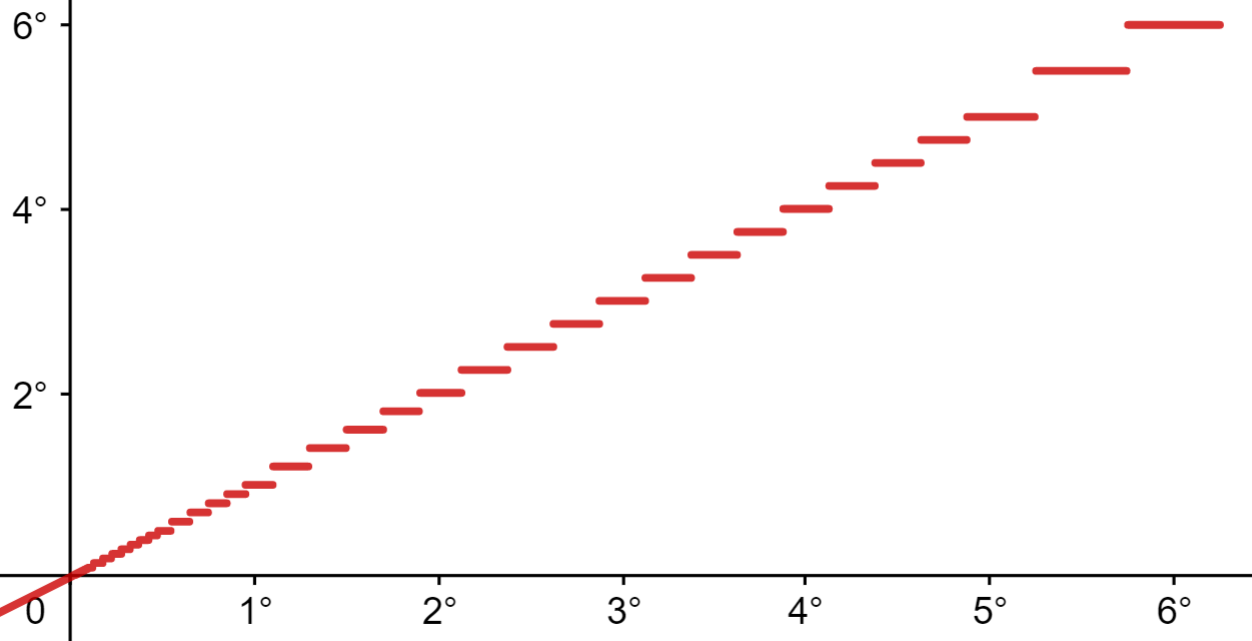
\includegraphics[width=0.5\textwidth]{img/lat-long-discretization}
        \end{center}
        \caption{Funkcja dyskretyzacji kąta}
    \end{figure}

    \item
    \Large\emph{[geolocation-service]} - \textbf{selectByGeohash}\normalsize\\
    \emph{Geohash} w dużym skrócie jest funkcją dyskretyzacji powierzchni globu.
    Zamienia długość i szerokość geograficzną na identyfikator wycinka Ziemi, w którym się znajduje.
    W ten sposób poindeksowane są obiekty w tabeli \cw{GEOLOCATION}. Znacznie przyspiesza to zapytania punkty w zadanym obszarze.

    \item
    \Large\emph{[geolocation-service]} - \textbf{klasteryzacja}\normalsize\\
    Wykonywana jest po stronie backendu, aby nie obarczać tym zadaniem aplikacji mobilnej. 
    W zależności od stopnia przybliżenia wykorzystywany jest jeden z trzech algorytmów:

    \begin{itemize}
        \item
        \textbf{\emph{Geohash}} - klasteryzacja na podstawie \emph{Geohash}'u

        \item
        \textbf{\emph{DBSCAN}} - algorytm opierający się na gęstości punktów

        \item
        \textbf{\emph{k-means}} - kieruje się średnią odległością dzielącą punkty

    \end{itemize} 
    

    \item
    \Large{\emph{[spot-service]} - \textbf{GET /spots/filter-ids} (spotFilters)}\normalsize\\
    \emph{Geolocation-service} zwraca sklasteryzowane identyfikatory obiektów w zadanym obszarze.
    Teraz pora na filtrowanie tego zbioru po zadanych w zapytaniu parametrach.
    To zadanie należy do \emph{spot-service}. Zwraca on zbiór identyfikatorów spełniających kryteria.

    \item
    \Large{\emph{[geolocation-service]} - \textbf{GET /geolocations}/\{uid\}}\normalsize\\
    W przypadku gdy grupa identyfikatorów stanowiąca klaster zostanie zredukowana po filtrowaniu do pojedynczego punktu, wypada skorygować jego koordynaty.
    Wołany jest wtedy \emph{geolocation-service} by pozyskać dokładny punkt.

    \item
    \Large{\emph{[spot-service]} - \textbf{GET /spots}/\{uid\}}\normalsize\\
    Każdy pojedynczy punkt dekorowany jest skojarzonymi danymi spotu, klastry są pomijane.

    \item
    \Large\emph{[map-supplier]} - \textbf{MapSupplierResponse}\normalsize
    \begin{itemize}
        \item
        \textbf{\emph{matchedRectangle}} - użyty obszar po dyskretyzacji

        \item
        \textbf{\emph{points}} - wynikowe obiekty - klastry lub pojedyncze spoty

    \end{itemize} 
    


\end{enumerate}



